\chapter{\texorpdfstring{Search for extended Higgs sector signatures in $\PGt^+\PGt^-\PGt^+\PGt^-$ final states}{Search for extended Higgs sector signatures in tautautautau final states}}
\chaptermark{Extended Higgs sector search}  
\thispagestyle{plain}  % First page has default style
\pagestyle{chapterpages}
\label{Section:Chapter_4tau}
\minitoc

\section{Introduction}

Motivated by the theoretical considerations and the particularly intriguing measurement of the muon anomalous magnetic moment discussed in Section~\ref{Section:Chapter2_gminus2}, this chapter presents a detailed analysis targeting final states with four tau leptons $\PGt$ through the process $Z^*\rightarrow\phi A\rightarrow4\PGt$.

The analysis explores a region of parameter space that remains largely unconstrained by existing collider searches. This is primarily because the production mode proceeds via an off-shell $Z^*$ boson. This circumvents the dominant SM Higgs production mechanisms, which are already tightly constrained by current LHC measurements. As such, this search offers unique sensitivity to scenarios in extended Higgs sectors that could otherwise evade detection.

This chapter provides a comprehensive description of the analysis strategy employed in the CMS experiment to probe this signature. 
\section{Data and Simulation}
\subsection{Collision data}

This search is based on pp collision data collected by the CMS detector during the 2016-2018 Run 2 data-taking period. The collisions were recorded at a centre-of-mass energy $\sqrt{s} = 13\TeV$ and the full dataset corresponds to an integrated luminosity of approximately $138\unit{fb}^{-1}$.

\subsection{Backgrounds}

This section provides a brief overview of the SM processes that can contribute to the four-$\PGt$ signal region. The aim is to provide an understanding of how different backgrounds can enter the selection through the presence of genuine or misidentified $\PGt$ leptons. The specific treatment of each background category is described in detail in Section~\ref{Section:Chapter6_Background_Modelling}.

\textit{Diboson} production, specifically $\PZ\PZ \to 4\PGt$, constitutes the primary irreducible background in this analysis. These events contain four genuine $\PGt$ leptons in the final state, matching the signal topology by construction. Although the cross section is small compared to other SM processes, the kinematic features of $\PZ\PZ$ events make them difficult to distinguish from potential signal. In addition, $\PZ\PZ$ events with mixed-flavour decays can contribute irreducibly when the final state includes leptonic tau decays, such as $\PGt_e\PGt_e\PGt_h\PGt_h$ or $\PGt_\mu\PGt_\mu\PGt_h\PGt_h$. In such cases, the prompt electrons or muons from the $\PZ$ decay could mimic the kinematic signature of non-prompt leptons originating from $\PGt$ decays.

The \textit{\ac{DY}} process, $\PZ/\gamma^* \to \ell^+\ell^-$, is one of the dominant backgrounds in di-$\PGt$ final states, producing genuine $\PGt^+ \PGt^-$ pairs in approximately one-third of events. Although its impact is reduced in four-$\PGt$ final states, it remains relevant in cases where two genuine $\PGt$ leptons are produced and are accompanied by jets from ISR or FSR. These jets can be misidentified as $\PGt_h$ candidates, resulting in final states that pass the selection for four reconstructed $\PGt$ leptons. In addition, prompt electrons or muons from $\PZ/\gamma^* \to \Pe^+\Pe^-$ or $\mu^+\mu^-$ decays may be misidentified as $\PGt_h$ candidates. When combined with one or more jets that are also misidentified as $\PGt_h$, such events can satisfy the four-$\PGt$ selection criteria. Feynman diagrams illustrating DY production with and without ISR/FSR are shown in Figure~\ref{Figure:Chapter6_DY}.

\begin{figure}[h]
    \centering
    % First row
    \begin{subfigure}{0.45\textwidth}
        \centering
        \begin{tikzpicture}
    \begin{feynman}
        \vertex at (0, 1.5) (i1) {\(q\)};
        \vertex at (0,-1.5) (i2) {\(\overline{q}\)};

        \vertex at (2,0) (a);
        \vertex at (4, 0) (b);

        \vertex at (6.15, 1.5) (c) {\(\ell^-\)};
        \vertex at (6,-1.5) (d) {\(\ell^+\)};

        \vertex at (3,0.25) () {\(Z/\gamma^*\)};

        \diagram*{
            (i1) -- [fermion] (a) -- [fermion] (i2),
            (a) -- [photon] (b),
            (d) -- [fermion] (b) -- [fermion] (c),
        };
    \end{feynman}
\end{tikzpicture}
        \caption{}
    \end{subfigure}
    \hfill
    \begin{subfigure}{0.45\textwidth}
        \centering
        \begin{tikzpicture}
    \begin{feynman}
        \vertex at (0, 1.5) (i1) {\(q\)};
        \vertex at (0,-1.5) (i2) {\(\overline{q}\)};

        \vertex at (1.35, 0.5) (g1);
        \vertex at (2.5, 1.5) (g2);

        \vertex at (2,0) (a);
        \vertex at (4, 0) (b);

        \vertex at (6.15, 1.5) (c) {\(\ell^-\)};
        \vertex at (6,-1.5) (d) {\(\ell^+\)};

        \vertex at (3,0.25) () {\(Z/\gamma^*\)};

        \diagram*{
            (i1) -- [fermion] (a) -- [fermion] (i2),
            (g1) -- [gluon] (g2),
            (a) -- [photon] (b),
            (d) -- [fermion] (b) -- [fermion] (c),
        };
    \end{feynman}
\end{tikzpicture}
        \caption{}
    \end{subfigure}

    \caption[Examples of Feynman diagrams for Drell-Yan without partons and one parton originating from initial state radiation.]{Examples of Feynman diagrams for Drell-Yan \textbf{(a)} without partons and \textbf{(b)} one parton originating from ISR.}
    \label{Figure:Chapter6_DY}
\end{figure}

\textit{Top quark pair production} ($\ttbar \to b\overline{b}W^+W^-$) can also lead to four-$\PGt$ final states when both $\PW$ bosons decay leptonically via $\PW \to \PGt \nu_\PGt$. This results in two genuine $\PGt$ leptons, while additional jets from the top decays can be misidentified as $\PGt_h$ candidates, thereby mimicking the four-$\PGt$ topology. Misidentification can also occur between tau decay modes; for example, a $\PGt_h$ may be reconstructed as $\PGt_e$ or $\PGt_\mu$, or vice versa. Furthermore, similar to the DY background, prompt electrons or muons originating from $\PW \to e/\mu \nu$ decays may be misidentified as $\PGt_h$ candidates. In such cases, when combined with genuine $\PGt$ leptons or additional misidentified jets, multiple misidentifications may result in an event satisfying the four-$\PGt$ selection criteria.

\textit{W+jets} events can contribute to the four-$\PGt$ signal region when the $\PW$ boson decays via $\PW \to \PGt \nu_\PGt$, producing a genuine $\PGt$ lepton, and the accompanying jets are misidentified as $\PGt_h$ candidates. Similar to $\ttbar$, additional contributions arise from misidentified prompt electrons or muons. Since these events typically contain only one genuine lepton, multiple jet misidentifications are again required to satisfy the four-$\PGt$ selection.

\textit{QCD-induced multijet} events can enter the signal region when multiple jets are simultaneously misidentified as $\PGt_h$ candidates. These events may also feature non-prompt electrons or muons from the decay of hadrons. Such leptons can be misidentified as genuine prompt leptons and reconstructed as $\PGt_e$ or $\PGt_\mu$ candidates, thereby mimicking tau decays.

\textit{Diboson} processes such as $\PW\PW$ and $\PW\PZ$ may contribute to the four-$\PGt$ signal region when one or more of the bosons decay leptonically via $\PW/\PZ \to \PGt$, yielding up to two or three genuine $\PGt$ leptons. To satisfy the selection, the remaining $\PGt$ candidates must arise from jets misidentified as $\PGt_h$, originating either from hadronic boson decays (e.g., $\PW \to q \bar{q}'$, $\PZ \to q \bar{q}$) or from ISR or FSR. Misidentification of prompt electrons or muons as $\PGt_h$ candidates, following the same mechanism described for DY, $\ttbar$, and W+jets backgrounds, can also contribute. \textit{Triboson} production (e.g., $\PW\PW\PZ$, $\PZ\PZ\PZ$) can similarly yield multiple genuine leptons, including $\PGt$ decays, and may enter the signal region through analogous misidentification pathways.

Other subdominant processes also contribute. \textit{Single-top} production may yield a genuine $\PGt$ from a $\PW \to \PGt \nu_\PGt$ decay. Still, due to the typically low jet multiplicity in these events, additional $\PGt_h$ candidates must arise from misidentified jets, often requiring ISR or FSR. Finally, \textit{electroweak production} of $\PZ$ or $\PW$ bosons in association with jets (\eg VBF-like $\PZ + jj$) can resemble the signal topology when real or misidentified $\PGt$ candidates are produced alongside forward jets. 

Although many of the backgrounds discussed above are partially reducible through the application of $\PGt$ identification algorithms, lepton isolation requirements, and $b$-jet vetoes, these techniques are not fully efficient, and some backgrounds remain irreducible. To summarise, a common feature across many of these background processes is the presence of prompt electrons or muons that can be reconstructed as $\PGt_e$, $\PGt_\mu$ or $\PGt_h$ candidates. This, in combination with jet misidentification, enables events with fewer than four genuine $\PGt$ leptons to satisfy the selection criteria. The specific treatment, estimation, and validation of each background category are described in detail in Section~\ref{Section:Chapter6_Background_Modelling}.

The simulated background processes used in this analysis are summarised in Table~\ref{Table:Chapter6_SimulatedBackgrounds}.

{
\centering
\setlength{\LTpost}{-2ex}  % tighten space after table
\small  % one size smaller than normal
\begin{longtable}{llc}
\caption[Summary of the simulated Standard Model backgrounds, including their generators and precision, used in the extended Higgs sector search.]
{Summary of the simulated SM backgrounds, including their generators and precision, used in the search. The following generators were used: 
\MADGRAPH~\cite{MadGraph} for leading-order matrix element calculations; 
\POWHEG~v1.0~\cite{Powheg_0} and v2.0~\cite{Powheg_1,Powheg_2,Powheg_3} for next-to-leading order processes including $\ttbar$ and single top; 
and \MGvATNLO~\cite{MadGraph} for diboson and triboson production. 
Parton showering and hadronisation were performed with \PYTHIA~\cite{PYTHIA}.}
\label{Table:Chapter6_SimulatedBackgrounds} \\
\hline
\textbf{Process} & \textbf{Generators} & \textbf{Cross section $\sigma$ [pb]} \\
\hline \hline
\endfirsthead

\hline
\textbf{Process} & \textbf{Generators} & \textbf{Cross section $\sigma$ [pb]} \\
\hline \hline
\endhead

\hline
\multicolumn{3}{r}{\textit{Continued on next page}} \\
\endfoot

\hline
\endlastfoot
\rowcolor{verylightblue}
\textbf{Drell-Yan, $\PZ/\gamma^* \to \ell^+ \ell^-$ (LO)\hyperlink{DY_W-MLM}{$^1$}} & & \\
+ jets, $10 < m_{\ell \ell} < 50\GeV$ & \MADGRAPH, \PYTHIA & 15810.0 (LO), 18610.0 (NLO) \\
+ jets, $m_{\ell \ell} > 50\GeV$ & \MADGRAPH, \PYTHIA & 5379.0 (LO), 6077.2 (NNLO) \\
+1 jets\hyperlink{DY_W-Stitch}{$^2$}, $m_{\ell \ell} > 50\GeV$ & \MADGRAPH, \PYTHIA & 997.3 (LO) \\
+2 jets\hyperlink{DY_W-Stitch}{$^2$}, $m_{\ell \ell} > 50\GeV$ & \MADGRAPH, \PYTHIA & 347.0 (LO)\\
+3 jets\hyperlink{DY_W-Stitch}{$^2$}, $m_{\ell \ell} > 50\GeV$ & \MADGRAPH, \PYTHIA & 126.4 (LO) \\
+4 jets\hyperlink{DY_W-Stitch}{$^2$}, $m_{\ell \ell} > 50\GeV$ & \MADGRAPH, \PYTHIA & 71.7 (LO) \\

\arrayrulecolor{lightgray}\hline
\rowcolor{verylightblue}
\textbf{W+jets (LO)\hyperlink{DY_W-MLM}{$^1$}} & & \\
+ jets & \MADGRAPH, \PYTHIA & 52940.0 (LO), 61526.7 (NLO) \\
+1 jets\hyperlink{DY_W-Stitch}{$^2$} & \MADGRAPH, \PYTHIA & 9364.4 (LO) \\
+2 jets\hyperlink{DY_W-Stitch}{$^2$} & \MADGRAPH, \PYTHIA & 3168.6 (LO) \\
+3 jets\hyperlink{DY_W-Stitch}{$^2$} & \MADGRAPH, \PYTHIA & 1132.1 (LO) \\
+4 jets\hyperlink{DY_W-Stitch}{$^2$} & \MADGRAPH, \PYTHIA & 633.7 (LO) \\

\arrayrulecolor{lightgray}\hline
\rowcolor{verylightblue}
\textbf{\ttbar} & & \\
Fully hadronic & \POWHEG, \PYTHIA & 377.96 (NNLO)\\
Semi-leptonic & \POWHEG, \PYTHIA & 365.34 (NNLO)\\
Fully leptonic & \POWHEG, \PYTHIA & 88.29 (NNLO) \\

\arrayrulecolor{lightgray}\hline
\rowcolor{verylightblue}
\textbf{Single top} & & \\
t-channel ($t$) & \POWHEG, \PYTHIA & 136.02 (NNLO) \\
t-channel ($\overline{t}$) & \POWHEG, \PYTHIA & 136.02 (NNLO) \\
$t + W^-$ & \POWHEG, \PYTHIA & 35.60 (NNLO) \\
$t + W^+$ & \POWHEG, \PYTHIA & 35.60 (NNLO) \\

\arrayrulecolor{lightgray}\hline
\rowcolor{verylightblue}
\textbf{Diboson} & & \\
$\PW \PZ \rightarrow \ell \, \nu \, \nu \, \nu$  & \MCATNLO, \PYTHIA & 3.416 (NLO) \\
$\PW \PZ \rightarrow \ell \, \nu \, q \, q$        & \MCATNLO, \PYTHIA & 10.71 (NLO) \\
$\PW \PZ \rightarrow q \, q \, \ell \, \ell$            & \MCATNLO, \PYTHIA & 6.419 (NLO) \\
$\PW \PZ \rightarrow \ell \, \ell \,  \ell \, \nu $          & \MCATNLO, \PYTHIA & 5.213 (NLO) \\
$\PW \PW \rightarrow \ell \, \nu \, q \,q$        & \MCATNLO, \PYTHIA & 49.99 (NLO) \\
$\PW \PW \rightarrow \ell \, \nu \, \ell \, \nu$        & \POWHEG, \PYTHIA & 11.09 (NLO) \\
$\PZ \PZ \rightarrow \ell \, \ell \, \nu \, \nu$         & \POWHEG, \PYTHIA & 0.9740 (NLO) \\
\arrayrulecolor{lightgray}\hline
$\text{H}_{\text{VBF}} \rightarrow ZZ \rightarrow \ell \, \ell \, \ell \, \ell $ & \POWHEG, \PYTHIA & $1.040e^{-3}$ (NLO) \\
$\text{ggH} \rightarrow ZZ \rightarrow \ell \, \ell \, \ell \, \ell $ & \POWHEG, \PYTHIA & $1.333e^{-2}$ (NLO)\\
$qq \rightarrow ZZ \rightarrow \ell \, \ell \, \ell \, \ell $ & \POWHEG, \PYTHIA & 1.325 (NLO)\\
$gg \rightarrow ZZ \rightarrow e \, e \, \PGt \, \PGt $ & \PYTHIA & $3.194e^{-3}$ (NLO)\\
$gg \rightarrow ZZ \rightarrow \mu \, \mu \, \PGt \, \PGt $ & \PYTHIA & $3.194e^{-3}$ (NLO)\\
$gg \rightarrow ZZ \rightarrow \mu \, \mu \, \mu \, \mu $ & \PYTHIA & $1.585e^{-3}$ (NLO)\\
$gg \rightarrow ZZ \rightarrow \PGt \, \PGt \, \PGt \, \PGt $ & \PYTHIA & $1.585e^{-3}$ (NLO)\\

\arrayrulecolor{lightgray}\hline
\rowcolor{verylightblue}
\textbf{Triboson} & & \\
$\PW \PW \PZ $ & \MCATNLO, \PYTHIA & 0.1707 (NLO)\\
$\PW \PZ \PZ $ & \MCATNLO, \PYTHIA & 0.0571 (NLO)\\
$\PW \PW \PW $ & \MCATNLO, \PYTHIA & 0.2158 (NLO)\\
$\PZ \PZ \PZ $ & \MCATNLO, \PYTHIA & 0.0148 (NLO)\\

\arrayrulecolor{lightgray}\hline
\rowcolor{verylightblue}
\textbf{Pure Electroweak} & & \\
$\PW^+ \to \ell^+ \nu$ + 2 jets & \MADGRAPH, \PYTHIA & 25.62 (LO)\\
$\PW^- \to \ell^- \nu$ + 2 jets & \MADGRAPH, \PYTHIA & 20.25 (LO)\\
$\PZ \to \ell \ell$ + 2 jets & \MADGRAPH, \PYTHIA & 3.987 (LO)\\

\arrayrulecolor{black}\hline
\end{longtable}
}
\vspace{0.5em}
\noindent\begin{minipage}{\linewidth}
\footnotesize
\hypertarget{DY_W-MLM}{}$^{1}$ MLM jet matching scheme~\cite{MLM} is employed to avoid double counting between jets produced at the matrix element level and those generated during parton showering.\\
\hypertarget{DY_W-Stitch}{}$^{2}$ To improve statistical precision, exclusive samples with fixed jet multiplicities are generated using the MLM scheme. These are stitched with inclusive samples to reproduce the overall cross-section and kinematic distributions accurately.
\end{minipage}

% For \ac{NLO} simulations, however, the MLM scheme is incompatible with the negative event weights that naturally arise. In such cases, the FxFx jet merging scheme~\cite{FxFx} is used instead. 


% Although the background samples are generated at LO or NLO, the comparison of simulated events to data is performed using higher-order theoretical cross-sections. Specifically, $\PW$+jets, Z+jets, $\ttbar$, and single top quark events in the tW channel are normalised using \ac{NNLO} cross-sections~\cite{HighOrder_XS_1,HighOrder_XS_2,HighOrder_XS_3}, while single top and diboson events are normalised to cross-sections calculated at NLO~\cite{HighOrder_XS_3,HighOrder_XS_4,HighOrder_XS_5}.

\subsection{Modelling of Signal Processes}
\label{Section:Chapter6_SignalModelling}

Signal templates targeting the process $Z^* \to \phi A \to \PGt^+\PGt^-\PGt^+\PGt^-$ are modelled in the \MCATNLO (version 2.6.5) framework~\cite{MadGraph,FxFx} at NLO accuracy in QCD. The event generation is performed in the five-flavour scheme using the NNPDF3.1 PDFs~\cite{NNPDF}. Parton showering, hadronisation, and $\PGt$ lepton decays are simulated using \PYTHIA (version 8.230)~\cite{PYTHIA}, with the underlying event modelled according to the CP5 tune~\cite{CP5_Tune}. To reflect realistic running conditions, additional pp interactions are overlaid on simulated events according to the distribution observed in the Run 2 data-taking period. The detector response is simulated using the \GEANTfour-based CMS framework~\cite{GEANT4}, and events are reconstructed with the same software configuration as applied to collision data.

A two-dimensional mass grid is defined to ensure sensitivity across the allowed phase space. All masses are expressed in units of~\GeV. The grid consists of combinations of $m_A$ and $m_\phi$ as follows:

\begin{itemize}
    \item $m_A$: 40, 50, 60, 70, 80, 90, 100, 125, 140, 160, 200, 250, 300, 400, 600
    \item For each $m_A$, the following $m_\phi$ values are considered:
    \begin{itemize}
        \item $m_A = 40$--$90$: 60, 70, 80, 90, 100, 110, 125, 140, 160, 180, 200, 250, 300
        \item $m_A = 100$, $125$, $140$, $160$, $200$, $250$:  60-300 (as above), 400
        \item $m_A = 300$: 60–400 (as above), 600
        \item $m_A = 400$: 100, 110, 125, 140, 160, 180, 200, 250, 300, 400, 600
        \item $m_A = 600$: 400, 600, 800
    \end{itemize}
\end{itemize}

The signal is simulated under the \textit{alignment limit} of the 2HDM, consistent with current experimental constraints on the couplings of the observed Higgs boson. The specific scenario is dynamically selected at each mass point depending on the value of $m_\phi$:
\begin{itemize}
    \item For $m_\phi > 125~\GeV$, the heavier CP-even scalar is identified as $\phi \equiv H$
    \item For $m_\phi \leq 125~\GeV$, the lighter CP-even scalar is identified as $\phi \equiv h$
\end{itemize}

Model parameters that do not significantly influence the kinematic properties of the final state, such as the charged Higgs mass and the soft $\mathbb{Z}_2$-breaking term, are fixed to values that preserve perturbative unitarity. This also ensures theoretical consistency~\cite{TypeX_2HDM}. Variations of these parameters within their allowed ranges have negligible impact on the resulting signal kinematics. They are therefore set according to the following prescription:
\begin{equation_pad}
m_{H^\pm} = m_\phi, \quad\quad m_{12}^2 = m_\phi^2 \sin\beta \cos\beta.
\end{equation_pad}

Figure~\ref{Figure:Chapter6_GenVisDistributions} illustrates the generator-level distributions of the visible di-$\PGt$ mass for selected combinations of $m_\phi$ and $m_A$. This observable is defined as the invariant mass computed using only the visible decay products of the two $\PGt$ leptons (\ie excluding neutrinos). These examples illustrate the primary kinematic characteristics of the signal across the mass grid.

\begin{figure}[h]
        \centering
        % First row
        \begin{subfigure}[b]{0.7\textwidth}
            \centering
            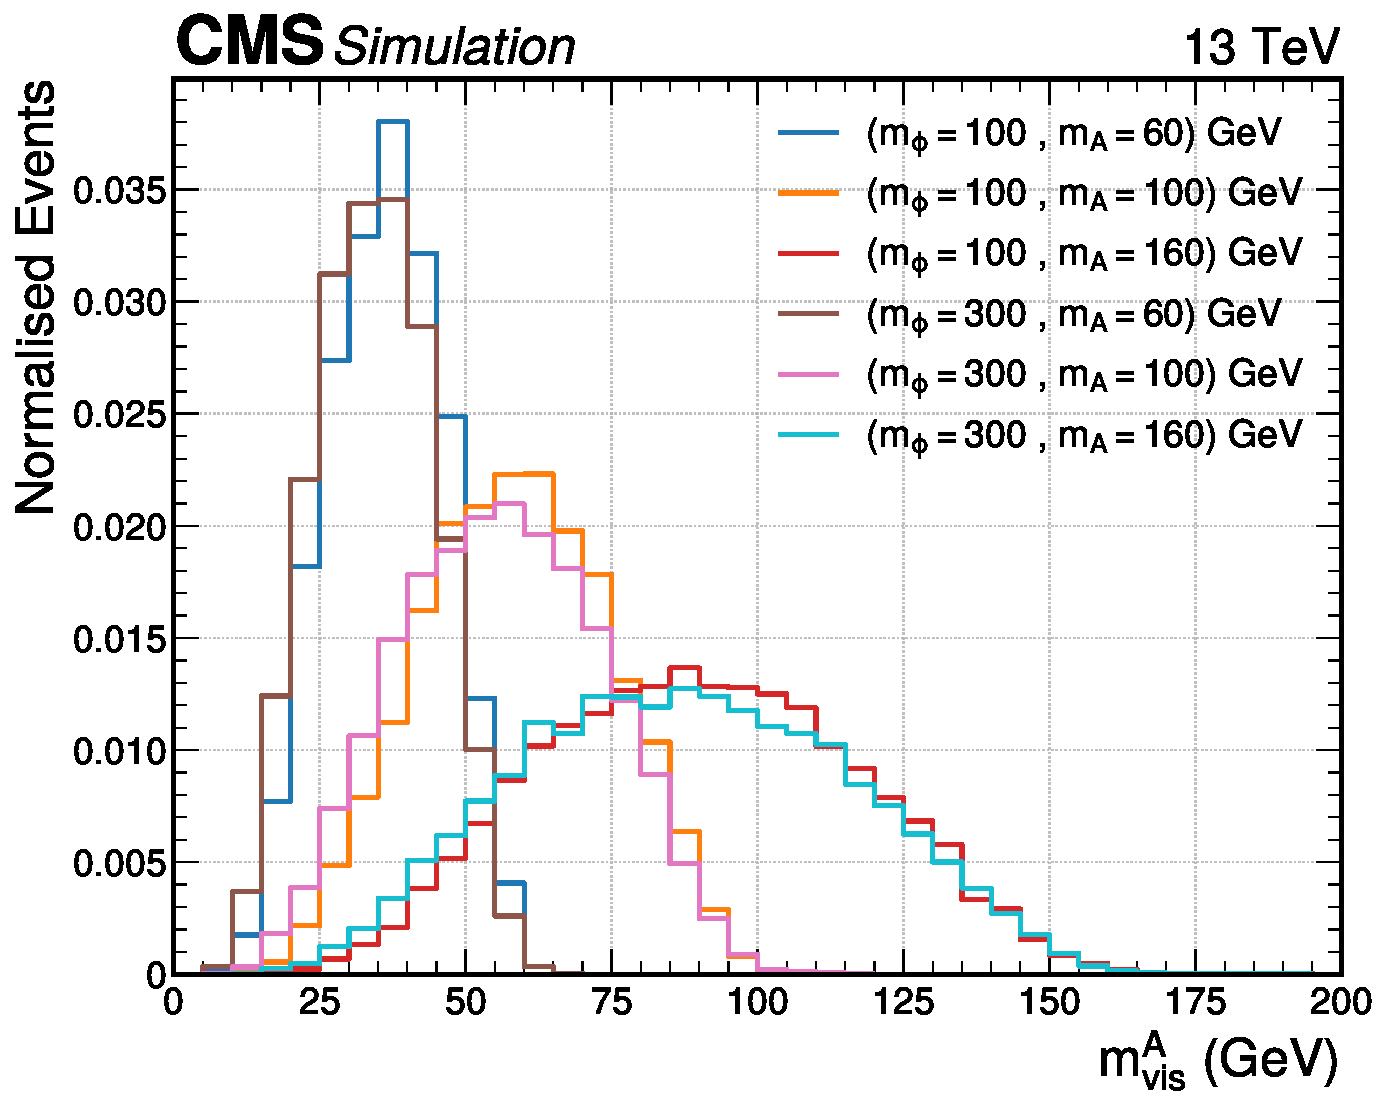
\includegraphics[width=\textwidth]{Figures/Chapter6/mvis_A.pdf}
            \caption{}
        \end{subfigure}
        \hfill
        \begin{subfigure}[b]{0.7\textwidth}
            \centering
            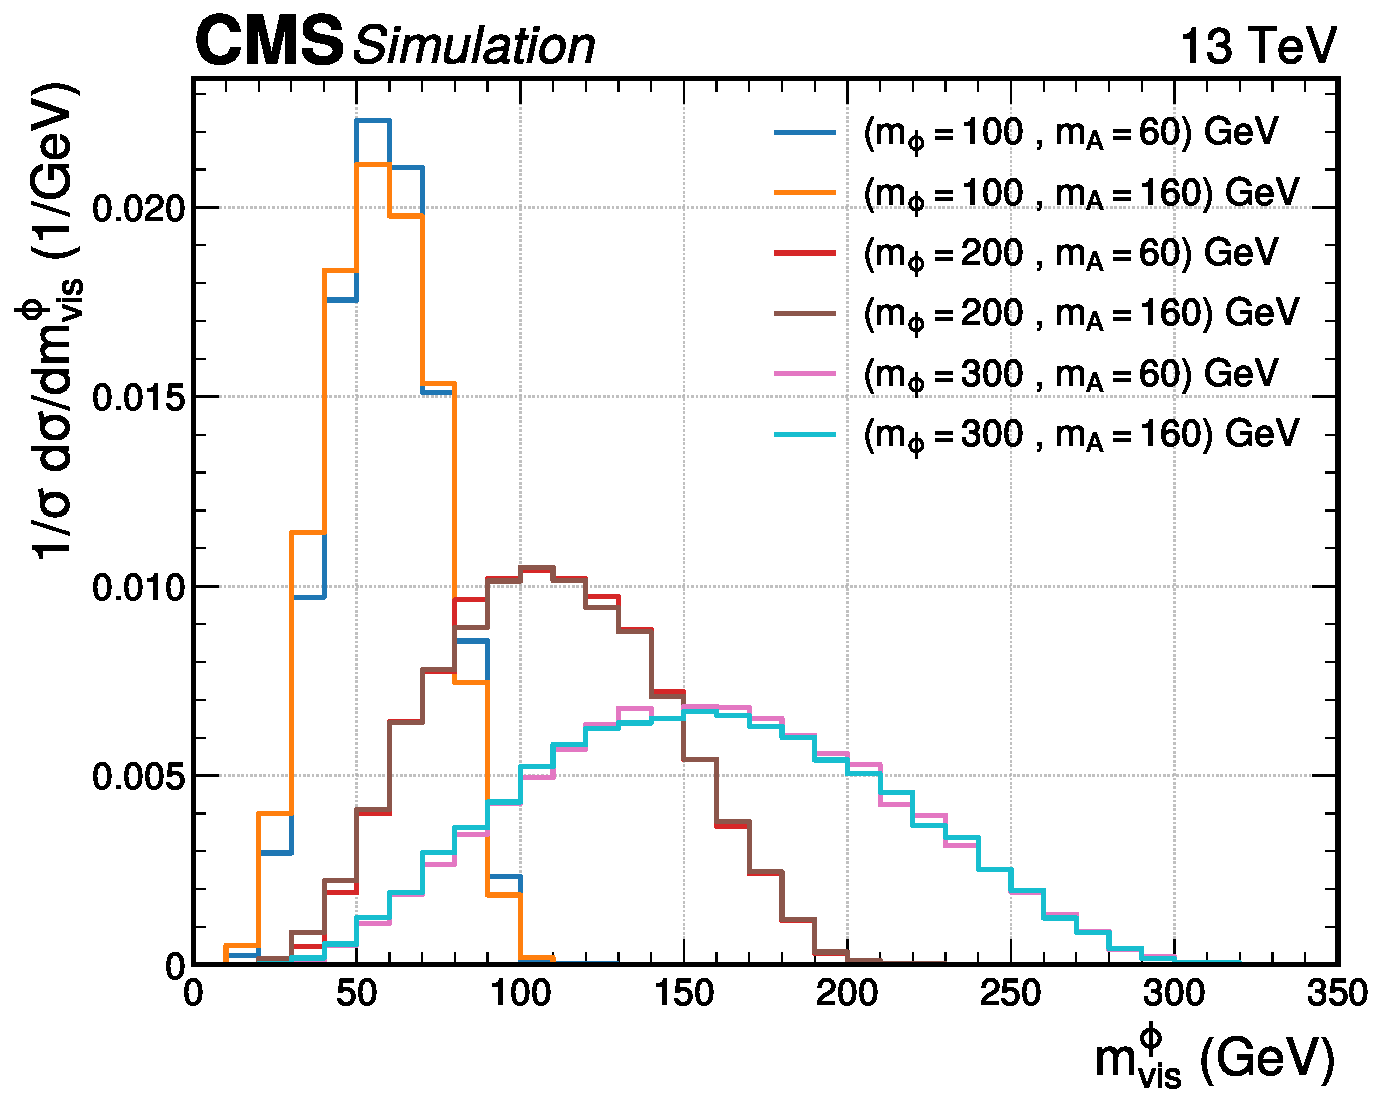
\includegraphics[width=\textwidth]{Figures/Chapter6/mvis_phi.pdf}
            \caption{}
        \end{subfigure}
    \caption[Generator-level visible mass distributions for different mass combinations of $\phi$ and A.]{Generator-level distributions of the visible di-$\PGt$ mass for selected combinations of $m_A$ and $m_\phi$. The visible mass is computed using only the decay products of the two $\PGt$ leptons, excluding neutrinos. Distributions are shown for scans over \textbf{(a)} $m_A$ and \textbf{(b)} $m_\phi$.}
    \label{Figure:Chapter6_GenVisDistributions}
\end{figure}
\clearpage

\subsubsection{Production Cross Sections and Branching Fractions}

The production cross section is computed at NLO and, within the alignment limit, is independent of $\tan\beta$. It varies across the mass plane, ranging from approximately $10~\unit{fb}$ at $(m_\phi, m_A) = (100, 60)~\GeV$ to $650~\unit{fb}$ at $(300, 160)~\GeV$. These values are summarised in Figure~\ref{Figure:Chapter6_ProductionXS}, which shows the cross section as a function of the two mass parameters in the alignment scenario.

\begin{figure}[h]
  \centering
  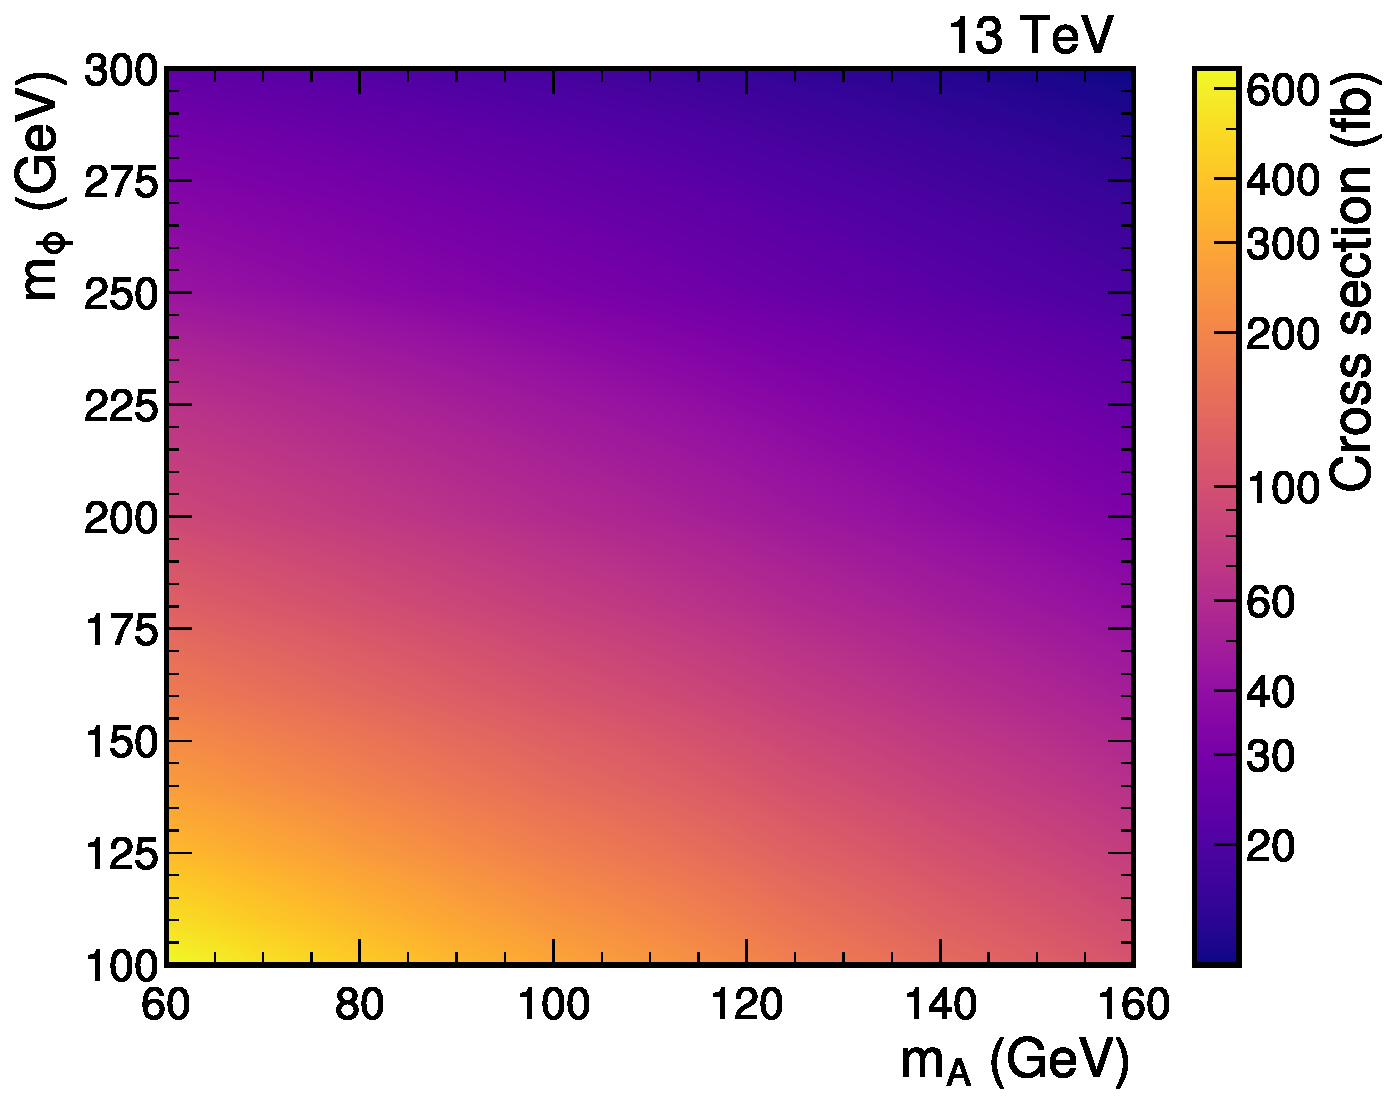
\includegraphics[width=0.85\textwidth]{Figures/Chapter6/Production_XS.pdf}
    \caption[Production cross sections for $Z^* \to \phi A$ in the alignment limit.]{Production cross sections for $Z^ \to \phi A$ in the alignment limit at NLO, shown as a function of $m_\phi$ and $m_A$. The values are interpolated over a grid of simulated mass combinations.}
  \label{Figure:Chapter6_ProductionXS}
\end{figure}

Outside the alignment limit, the cross section acquires dependence on the scalar mixing angle. Specifically:
\begin{itemize}
    \item It scales with $\sin^2(\beta - \alpha)$ when $\phi \equiv H$ ($m_\phi > 125~\GeV$),
    \item It scales with $\cos^2(\beta - \alpha)$ when $\phi \equiv h$ ($m_\phi \leq 125~\GeV$).
\end{itemize}

The decay branching ratios of $\phi$ and $A$ into $\PGt^+\PGt^-$ are computed using \textsc{2HDECAY}~\cite{2HDECAY}. In the alignment limit, the $\PGt^+\PGt^-$ branching ratio of $A$ remains close to unity for $\tan\beta \gtrsim 2$, but decreases rapidly at lower $\tan\beta$, where hadronic decays such as $A \to b\bar{b}$ become dominant. A similar pattern holds for $\phi \to \PGt^+\PGt^-$, except when the mass difference $m_\phi - m_A$ exceeds $m_Z$. In such cases, the decay $\phi \to ZA$ becomes kinematically accessible and can significantly suppress the di-$\PGt$ branching fraction, even at large $\tan\beta$. These features are illustrated in Figure~\ref{Figure:Chapter6_BranchingFractions}, which shows representative branching fraction maps for selected mass configurations. 

\begin{figure}[h]
        \centering
        % First row
        \begin{subfigure}[b]{0.49\textwidth}
            \centering
            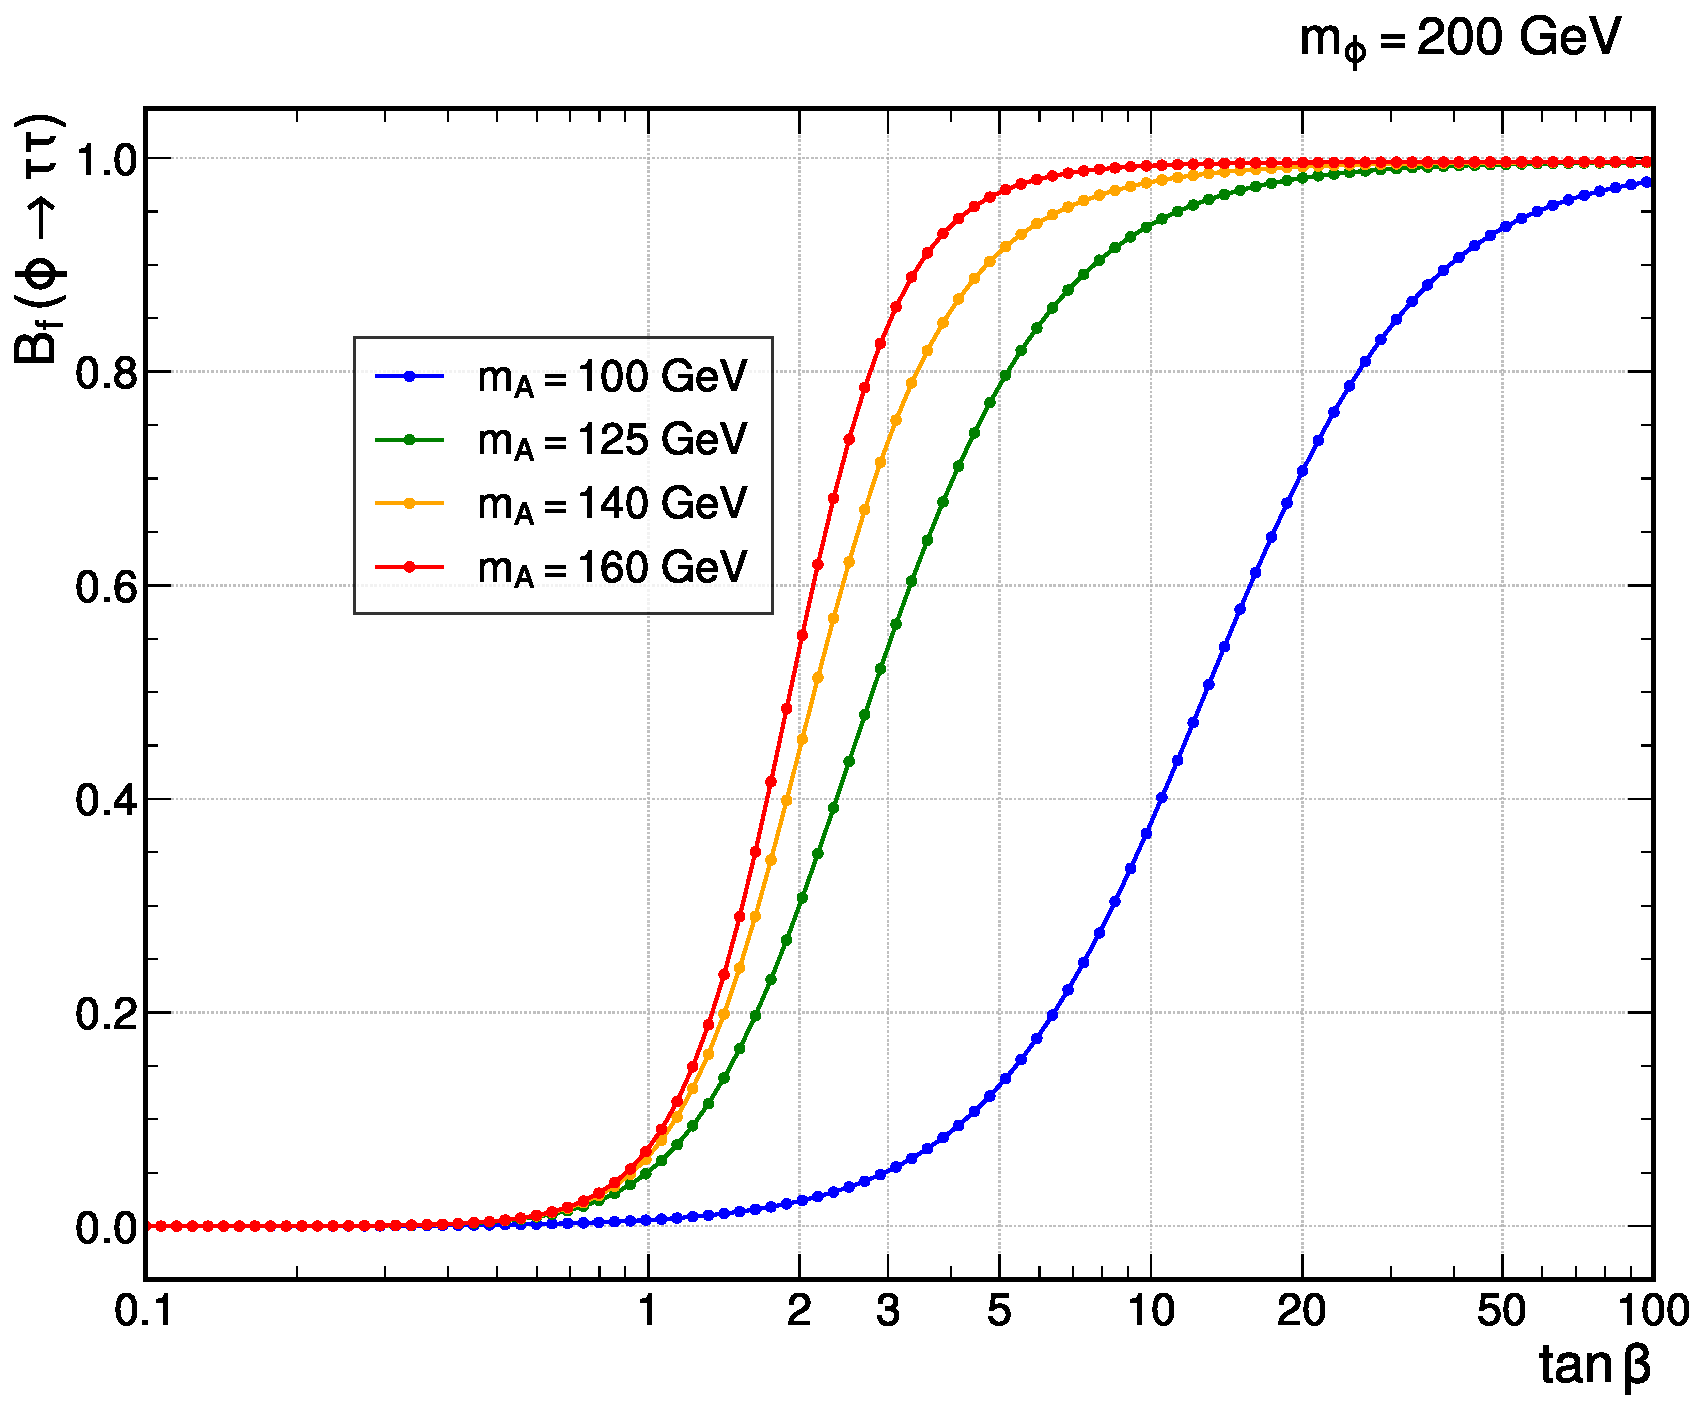
\includegraphics[width=\textwidth]{Figures/Chapter6/Phi_BR.pdf}
            \caption{}
        \end{subfigure}
        \begin{subfigure}[b]{0.49\textwidth}
            \centering
            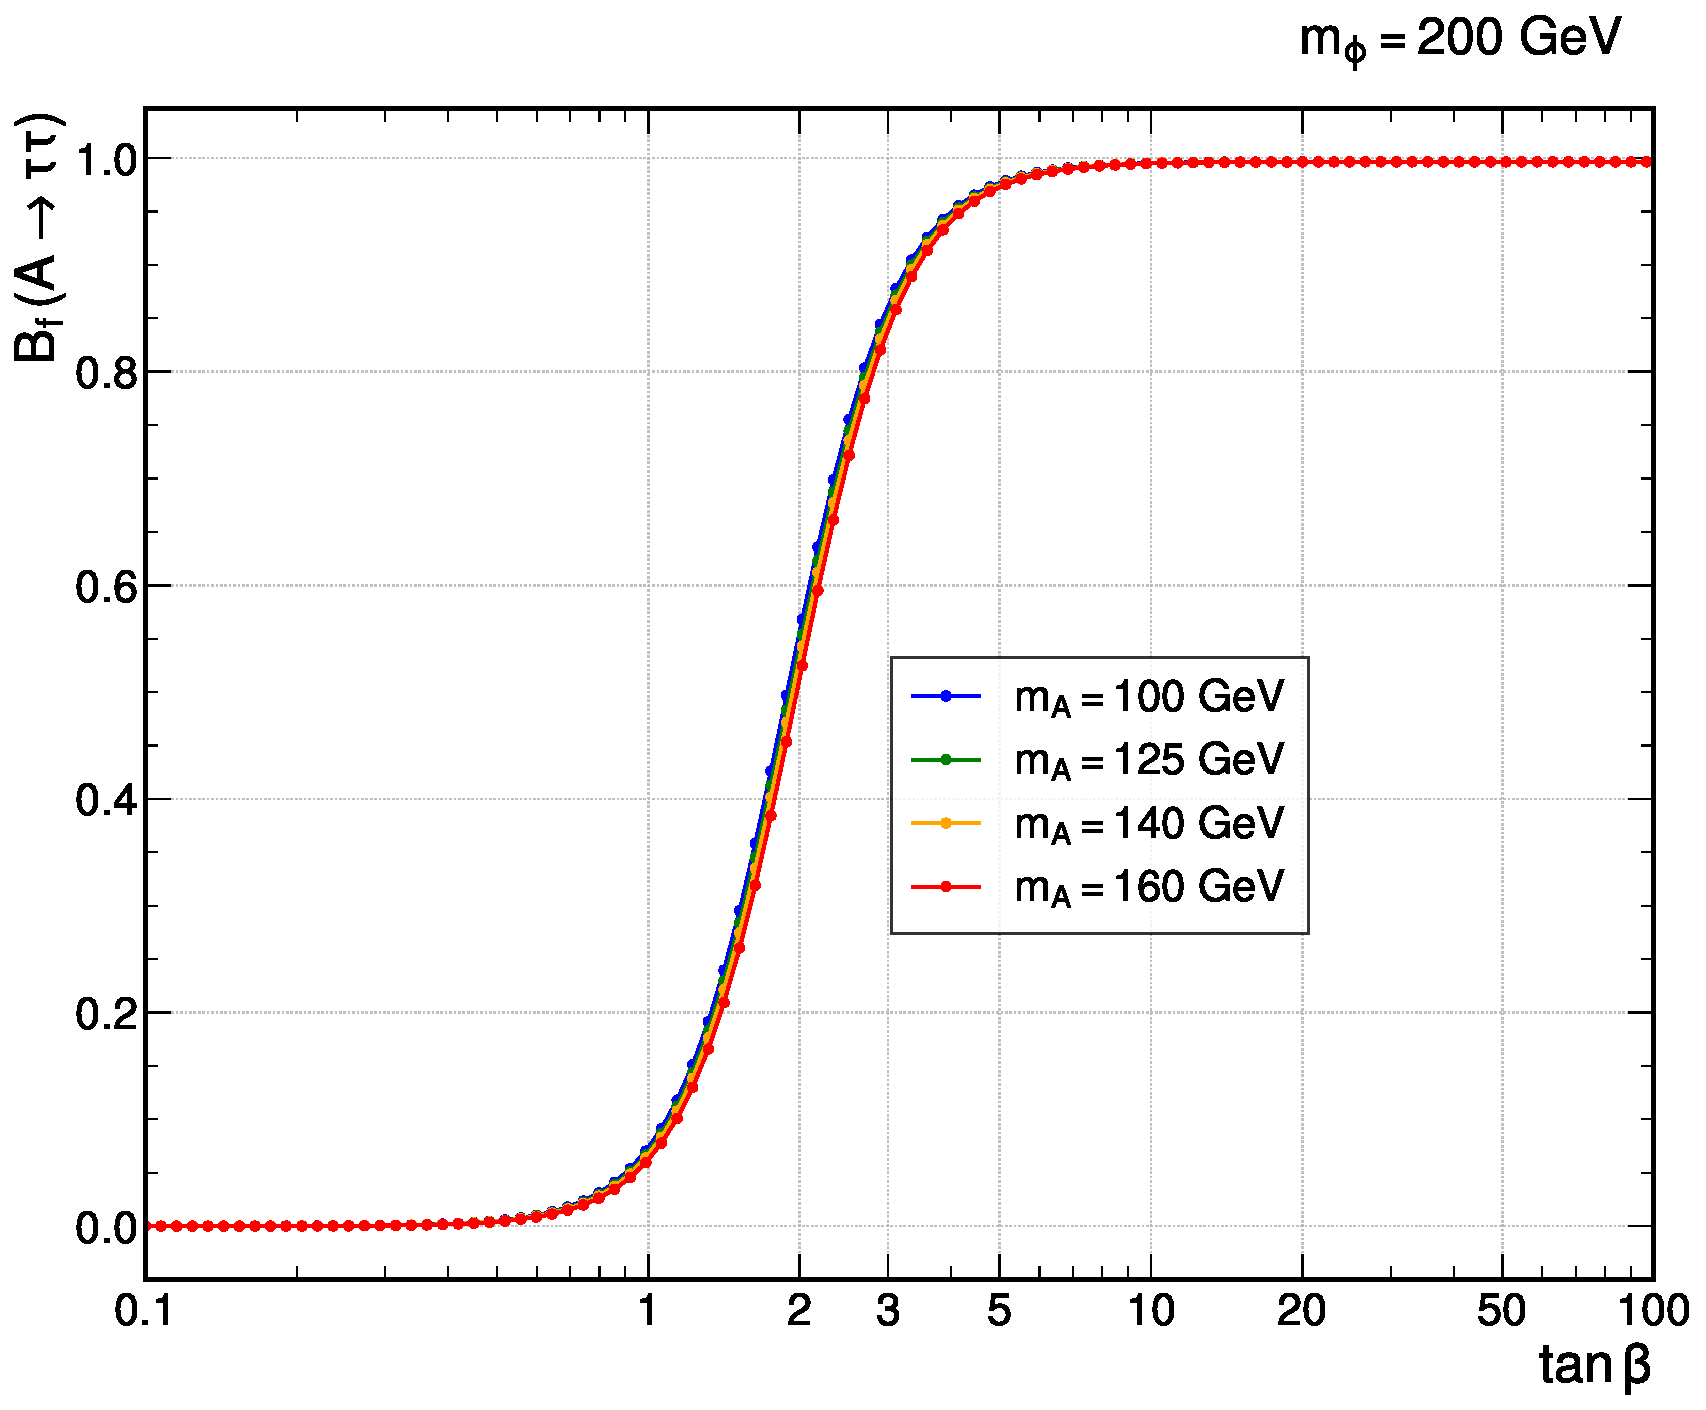
\includegraphics[width=\textwidth]{Figures/Chapter6/A_BR.pdf}
            \caption{}
        \end{subfigure}
    \caption[Branching fractions of $\phi$ and $A$ to $\PGt^+\PGt^-$ for selected mass combinations.]{Branching fractions of \textbf{(a)} $\phi \to \PGt^+\PGt^-$ and \textbf{(b)} $A \to \PGt^+\PGt^-$ as a function of $m_\phi$ and $m_A$, computed using \textsc{2HDECAY} in the alignment limit.}
    \label{Figure:Chapter6_BranchingFractions}
\end{figure}

\section{Event selection strategy}
\label{sec:ObjectAndEventSelections}

Having established the motivation, signal modelling, and background composition, this section describes the strategy used to identify candidate $Z^* \to \phi A \to 4\PGt$ events. The final states considered consist of four tau leptons, each of which may decay either leptonically ($\PGt_e$ and $\PGt_{\mu}$) or hadronically ($\PGt_h$). Figure~\ref{Figure:Chapter6_4tau_decayModes_BF} displays a pie chart of the most frequent $4\PGt$ final states, constructed by enumerating all combinations of leptonic and hadronic tau decays and summing their relative contributions. The dominant modes are those containing two or more hadronic taus, which together comprise 87.1\% of all four-tau decays. These channels form the focus of the analysis. In contrast, Table~\ref{Table:Chapter6_4tau_decayModes_BF_Other} summarises rarer final states that are not considered in the analysis.

\begin{figure}[h]
  \centering
  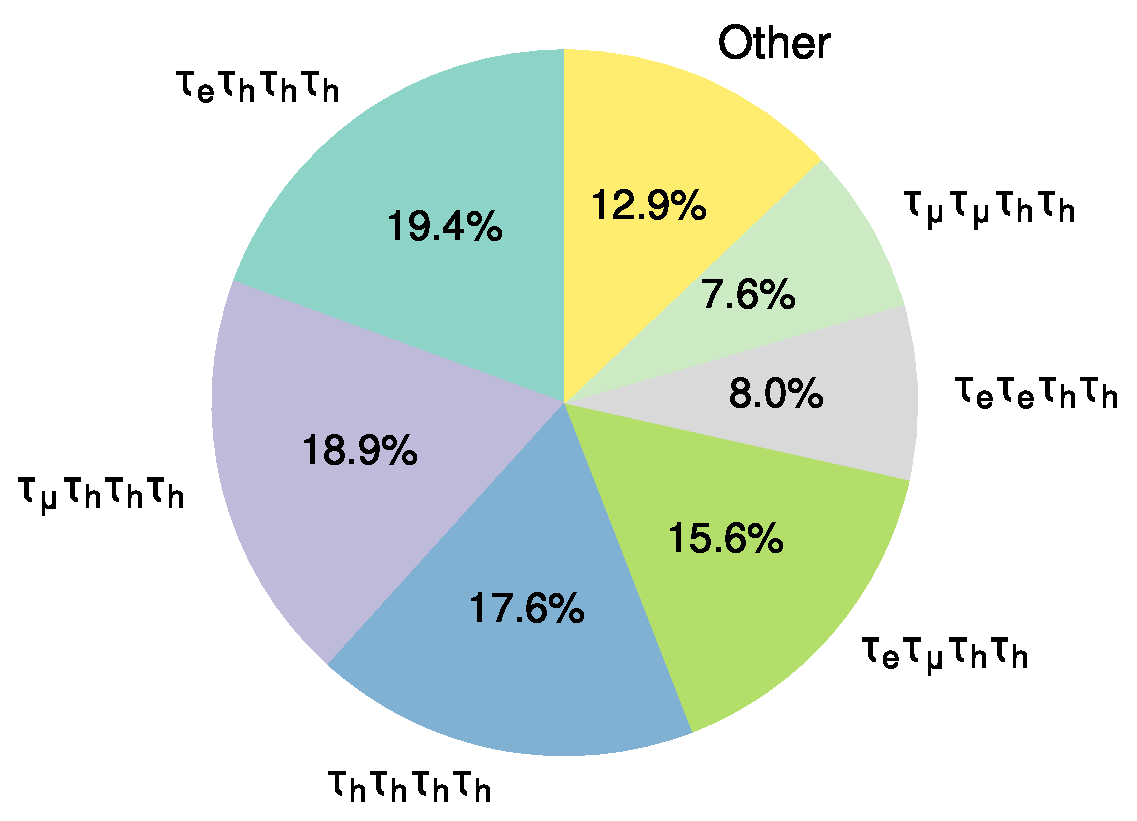
\includegraphics[width=0.8\textwidth]{Figures/Chapter6/pie_BF.pdf}
    \caption[Branching fractions of the dominant four-$\PGt$ decay modes.]
    {Branching fractions of the most frequent $4\PGt$ final states, constructed by enumerating all combinations of leptonic ($\PGt_e$, $\PGt_{\mu}$) and hadronic ($\PGt_h$) tau decays.}
  \label{Figure:Chapter6_4tau_decayModes_BF}
\end{figure}

\begin{table}[h]
\centering
\renewcommand{\arraystretch}{1.5} % Increase row height
\setlength{\tabcolsep}{12pt} % Increase column width
\arrayrulecolor{black} % Ensure outer border is black
\begin{tabular}{|c|c|}
\hline
Decay Mode                  & Branching Fraction {[}\%{]} \\ \hline \hline
$\PGt_e \PGt_e \PGt_{\mu} \PGt_h$             & 4.3 \\ 
\arrayrulecolor{lightgray} \hline
$\PGt_e \PGt_{\mu} \PGt_{\mu} \PGt_h$                    & 4.2 \\ 
\arrayrulecolor{lightgray} \hline
$\PGt_e \PGt_e \PGt_{e} \PGt_h$                        & 1.5  \\ 
\arrayrulecolor{lightgray} \hline
$\PGt_{\mu} \PGt_{\mu} \PGt_{\mu} \PGt_h$                  & 1.4  \\ 
\arrayrulecolor{lightgray} \hline
$\PGt_e \PGt_e \PGt_{\mu} \PGt_{\mu}$             & 0.6  \\ 
\arrayrulecolor{lightgray} \hline
$\PGt_e \PGt_e \PGt_{e} \PGt_{\mu}$                     & 0.4  \\ 
\arrayrulecolor{lightgray} \hline
$\PGt_e \PGt_{\mu} \PGt_{\mu} \PGt_{\mu}$             & 0.4  \\ 
\arrayrulecolor{lightgray} \hline
$\PGt_e \PGt_e \PGt_{e} \PGt_e$                  & 0.1  \\ 
\arrayrulecolor{lightgray} \hline
$\PGt_{\mu} \PGt_{\mu} \PGt_{\mu} \PGt_{\mu}$                  & 0.1  \\ 
\arrayrulecolor{black} \hline
\end{tabular}
\caption[Branching fractions of subdominant four-$\PGt$ decay modes]{Branching fractions of subdominant four-$\PGt$ final states, involving three or more leptonic $\PGt$ decays.}
\label{Table:Chapter6_4tau_decayModes_BF_Other}
\end{table}

In addition to focusing on the dominant final states with two or more hadronic taus, the analysis includes an orthogonal $\PGt_h\PGt_h\PGt_h$ channel. This channel targets events where one $\PGt_h$ in the fully hadronic $\PGt_h\PGt_h\PGt_h\PGt_h$ decay mode fails to be reconstructed, often due to limited trigger and identification efficiencies or high $p_\text{T}$ thresholds. In total, seven final states are retained for the analysis. Furthermore, a $\tau_\mu\tau_\mu\tau_\mu\tau_\mu$ control region is used to constrain the background prediction; this region is discussed in more detail in Section~\ref{Section:Chapter6_Background_Modelling}.

\subsection{Triggering}

Identifying events with four tau leptons poses a challenge, as there is no dedicated trigger that directly targets this specific final state. Instead, the selection relies on a combination of existing triggers designed to capture subsets of the decay products. The triggers considered include double-electron, double-muon, electron–muon, and single-lepton (electron or muon) triggers, as well as cross-triggers involving an electron or muon paired with a hadronic tau ($\tau_h$), specifically $e+\tau_h$ and $\mu+\tau_h$. Single-$\tau_h$ triggers, although available, are not used due to their high $p_T$ thresholds, which are too restrictive for the phase space targeted by this analysis. Cross-triggers and electron–muon triggers were also evaluated but found to offer negligible gains in signal acceptance. Therefore, they are excluded to simplify the calculation of trigger efficiencies. The set of triggers used, along with the relevant online $p_\text{T}$ thresholds for each data-taking period, is summarised in Table~\ref{Table:Chapter6_TriggerThresholdsExpanded}.

\begin{table}[h]
\centering
\renewcommand{\arraystretch}{1.5}
\setlength{\tabcolsep}{12pt} % Increase column width
\begin{tabular}{|c|cc|cc|cc|}
\hline
\multirow{3}{*}{\text{Trigger}} 
& \multicolumn{6}{c|}{$p_\text{T}$ \text{Threshold (GeV)}} \\ \cline{2-7}
& \multicolumn{2}{c|}{\text{2016}} & \multicolumn{2}{c|}{\text{2017}} & \multicolumn{2}{c|}{\text{2018}} \\ \cline{2-7}
& \text{Obj$_1$} & \text{Obj$_2$} & \text{Obj$_1$} & \text{Obj$_2$} & \text{Obj$_1$} & \text{Obj$_2$} \\ \hline \hline
Single Electron (e)                   & 26     & --     & 28     & --     & 33     & --     \\
\arrayrulecolor{lightgray} \hline
Single Muon ($\mu$)                       & 23     & --     & 25     & --     & 25     & --     \\
\arrayrulecolor{lightgray} \hline
Double Tau ($\PGt \PGt$)         & 40     & 40     & 40     & 40     & 40     & 40     \\
\arrayrulecolor{black} \hline
\end{tabular}
\caption{Table of minimum online $p_\text{T}$ thresholds (in GeV) for the triggers used in the analysis. Subcolumns refer to thresholds for the first and second trigger objects.}
\label{Table:Chapter6_TriggerThresholdsExpanded}
\end{table}

The specific trigger configuration used for each four-$\PGt$ final state is summarised in Table~\ref{Table:Chapter6_TriggersPerChannel}. These configurations are constructed as combinations of the single- and double-object triggers listed in Table~\ref{Table:Chapter6_TriggerThresholdsExpanded}. For each event category, the trigger is considered to have fired if at least one of the listed object combinations satisfies the corresponding online threshold. The use of logical OR($\lor$) between object pairs reflects the inclusive nature of the selection.

\begin{table}[h]
\centering
\renewcommand{\arraystretch}{1.5}
\setlength{\tabcolsep}{12pt}
\begin{tabular}{|c|c|}
\hline
\text{Channel} & \text{Trigger Configuration} \\ \hline \hline

$\tau_h\tau_h\tau_h\tau_h$ &  
$\tau_1\tau_2 \mathbin{\lor} \tau_1\tau_3 \mathbin{\lor} \tau_1\tau_4 \mathbin{\lor} \tau_2\tau_3 \mathbin{\lor} \tau_2\tau_4 \mathbin{\lor} \tau_3\tau_4$ \\ 
\arrayrulecolor{lightgray} \hline

$\tau_h\tau_h\tau_h$ &
$\tau_1\tau_2 \mathbin{\lor} \tau_1\tau_3 \mathbin{\lor} \tau_2\tau_3$ \\
\arrayrulecolor{lightgray} \hline

$\tau_e\tau_h\tau_h\tau_h$ &
$e_1 \mathbin{\lor} \tau_2\tau_3 \mathbin{\lor} \tau_2\tau_4 \mathbin{\lor} \tau_3\tau_4$ \\
\arrayrulecolor{lightgray} \hline

$\tau_\mu\tau_h\tau_h\tau_h$ &
$\mu_1 \mathbin{\lor} \tau_2\tau_3 \mathbin{\lor} \tau_2\tau_4 \mathbin{\lor} \tau_3\tau_4$ \\
\arrayrulecolor{lightgray} \hline

$\tau_e\tau_e\tau_h\tau_h$ &
$e_1 \mathbin{\lor} e_2 \mathbin{\lor} \tau_3\tau_4$ \\
\arrayrulecolor{lightgray} \hline

$\tau_\mu\tau_\mu\tau_h\tau_h$ &
$\mu_1 \mathbin{\lor} \mu_2 \mathbin{\lor} \tau_3\tau_4$ \\
\arrayrulecolor{lightgray} \hline

$\tau_e\tau_\mu\tau_h\tau_h$ &
$e_1 \mathbin{\lor} \mu_1 \mathbin{\lor} \tau_3\tau_4$ \\
\arrayrulecolor{lightgray} \hline

$\tau_\mu \tau_\mu \tau_\mu \tau_\mu$ &
$\mu_1 \mathbin{\lor} \mu_2 \mathbin{\lor} \mu_3 \mathbin{\lor} \mu_4$ \\
\arrayrulecolor{black} \hline

\end{tabular}
\caption{Trigger configuration used for each four-$\PGt$ final state.}
\label{Table:Chapter6_TriggersPerChannel}
\end{table}

\subsection{Offline object selections}
\label{sec:ObjectSelection}

The object selections defined in this section are applied to reconstructed electrons, muons, and hadronically decaying tau candidates ($\tauh$), as discussed in Chapter~\ref{Section:Chapter4}. These selections are designed to suppress backgrounds from misidentified and non-prompt objects, while retaining high signal efficiency. 

To reduce contamination from PU vertices, all leptons and $\tauh$ candidates are required to be consistent with the PV. This is enforced by applying cuts on the transverse and longitudinal impact parameters. Electrons and muons must satisfy $|d_{xy}| < 0.045\unit{cm}$ and $|d_z| < 0.2\unit{cm}$, while $\tauh$ candidates are required to have $|d_z| < 0.2~\unit{cm}$. 

Electrons and muons are additionally required to be isolated from surrounding hadronic activity in order to suppress backgrounds from non-prompt sources. The relative isolation variables used for this purpose are defined in Chapter~\ref{Section:Chapter4}, Equations~\ref{Equation:Chapter4_PFIso_Electron} and~\ref{Equation:Chapter4_PFIso_Muon}. A threshold of $I^{e/\mu}_\text{PF} < 0.15$ is applied to electrons and muons. For $\tauh$ candidates, no explicit isolation requirement is imposed, as isolation information is already incorporated into the DeepTau discriminators.

The identification criteria for electrons and muons follow the strategies described in Chapter~\ref{Section:Chapter4}, where electrons are identified using a multivariate (BDT-based) discriminator targeting a 90\% signal efficiency, and muons are selected using the cut-based medium working point.  For hadronically decaying tau leptons, a looser identification strategy is employed to ensure sufficient event yields. Specifically, $\tauh$ candidates are required to pass the \texttt{Loose} working point of the $D_{\text{jet}}$ discriminator. To further reduce contamination from electrons and muons misidentified as tau candidates, the \texttt{VVLoose} working point of the $D_e$ discriminator and the \texttt{VLoose} working point of the $D_\mu$ discriminator are employed. These working points are chosen as an optimal compromise between background rejection and signal retention, tailored to the statistical requirements of the analysis. For reference, the corresponding DeepTau score thresholds for these working points are listed in Table~\ref{Table:Chapter4_DeepTau_WPs}.

To ensure consistency between online and offline event selection, reconstructed objects in each event must match the trigger-level objects responsible for firing the trigger. Matching is performed using a cone radius of $\Delta R < 0.5$. The number of required matches varies depending on the trigger configuration used for each final state, as summarised in Table~\ref{Table:Chapter6_TriggersPerChannel}. For channels using double-object triggers (e.g.\ $\tauh\tauh\tauh\tauh$), it is sufficient for any two reconstructed $\tauh$ candidates to match the corresponding trigger objects. In contrast, for channels that rely on single-lepton triggers (e.g.\ $e\,\tauh\tauh\tauh$), only one reconstructed object may be required to match the trigger, depending on which trigger path fired. For matched objects, stricter offline $p_T$ thresholds are applied to ensure operation within the plateau of the trigger efficiency turn-on curve: a margin of $+1\GeV$ is added for electrons and muons, and $+5\GeV$ for $\tauh$ candidates. Objects not responsible for triggering the event (i.e.\ unmatched) are allowed to satisfy looser baseline $p_T$ thresholds. This conditional approach ensures optimal signal acceptance while maintaining accurate modelling of the trigger response.

The complete set of offline object selection criteria is summarised in Table~\ref{Table:Chapter6_ObjectSelectionSummary}.

{
\setlength{\arrayrulewidth}{1pt}

% Move the caption BEFORE the table
\begin{table}[h]
\centering
\caption[Summary of baseline object selection criteria]{
Summary of baseline selection criteria applied to reconstructed electrons, muons, and hadronically decaying tau candidates ($\tauh$). Trigger-matched $p_T$ thresholds are defined relative to those in Table~\ref{Table:Chapter6_TriggerThresholdsExpanded}.
}
\label{Table:Chapter6_ObjectSelectionSummary}

\renewcommand{\arraystretch}{1.5}
\setlength{\tabcolsep}{12pt}
\arrayrulecolor{black}

\begin{tabular}{cccc}
\hline
\textbf{Criteria} & \textbf{Electron} & \textbf{Muon} & \textbf{Hadronic Tau} \\
\hline

$p_\text{T}$  & > $10\GeV$ & > $10\GeV$ & > $20\GeV$\\ 
\arrayrulecolor{lightgray} \hline

$p_\text{T}^{\text{Trigger}}$ & \multicolumn{3}{c}{$> \text{Table~\ref{Table:Chapter6_TriggerThresholdsExpanded}} + [1,\,1,\,5]$} \\
\arrayrulecolor{lightgray} \hline

$|\eta|$ & < $2.5$ & < $2.4$ & < $2.3$/$2.1$\hyperlink{DoubleTauTrigger-EtaCut}{$^1$} \\
\arrayrulecolor{lightgray} \hline

$|d_{xy}|$ & < $0.045\unit{cm}$ & < $0.045\unit{cm}$ & -- \\
\arrayrulecolor{lightgray} \hline

$|d_z|$ & < $0.2\unit{cm}$ & < $0.2\unit{cm}$ & < $0.2\unit{cm}$ \\
\arrayrulecolor{lightgray} \hline

Isolation & $I^e_\text{PF}$ < 0.15 & $I^\mu_\text{PF}$ < 0.15 & -- \\
\arrayrulecolor{lightgray} \hline

Identification
& \makecell{MVA w/o isolation\\(90\% WP)}
& Medium ID
& \makecell{
$D_{\text{jet}} \geq \texttt{Loose}$ \\
$D_{e} \geq \texttt{VVLoose}$ \\
$D_{\mu} \geq \texttt{VLoose}$
} \\
\arrayrulecolor{black} \hline
\end{tabular}
\vspace{0.5em}
\begin{minipage}{0.95\linewidth}
\raggedright
\footnotesize\hypertarget{DoubleTauTrigger-EtaCut}{}$^{1}$\,$|\eta| < 2.1$ is required for $\tauh$ candidates matched to trigger objects, reflecting the online trigger acceptance region.
\end{minipage}

\end{table}
}

\subsection{Event-level selections}
Beyond object-level requirements, additional criteria are imposed at the event level to enhance signal purity and enforce statistical orthogonality between final states. These include constraints on the number and charge of reconstructed objects, as well as vetoes on additional leptons and $b$-tagged jets. The complete set of event-level selections applied in each final state is summarised in Table~\ref{Table:Chapter6_Event_Channel_Selections}.

{
\setlength{\arrayrulewidth}{1pt}

% Move the caption BEFORE the table
\begin{table}[h]
\caption[Event-level selection requirements by channel.]{
Event-level selection criteria applied to each four-$\PGt$ final state. The table specifies the required number of electrons ($e$), muons ($\mu$), hadronic taus ($\tauh$), and $b$-tagged jets ($b_\text{jets}$), as well as the total charge requirement ($\sum q$) for the selected objects.}
\label{Table:Chapter6_Event_Channel_Selections}
\centering
\renewcommand{\arraystretch}{1.5}
\setlength{\tabcolsep}{12pt}
\arrayrulecolor{black}

\begin{tabular}{cccccc}
\hline
\textbf{Channel} & \textbf{$e$} & \textbf{$\mu$} & \textbf{$\tauh$} & \textbf{$b_\text{jets}$}\hyperlink{b-jet_selections}{$^1$} & \textbf{$\sum$\text{q}}\\
\hline

$\tau_h\tau_h\tau_h\tau_h$ &  0 & 0 & $\geq 4$ & $\geq 0$ & 0\\
\arrayrulecolor{lightgray} \hline

$\tau_h\tau_h\tau_h$ & 0 & 0 & 3 & $\geq 0$ & $\pm 1$\\
\arrayrulecolor{lightgray} \hline

$\tau_e\tau_h\tau_h\tau_h$ & 1 & 0 & $\geq3$ & $0$  & 0 \\
\arrayrulecolor{lightgray} \hline

$\tau_\mu\tau_h\tau_h\tau_h$ & 0 & 1 & $\geq 3$ & $0$ & 0 \\
\arrayrulecolor{lightgray} \hline

$\tau_e\tau_e\tau_h\tau_h$ & 2 & 0 & $\geq 2$ & $0$ & 0\\
\arrayrulecolor{lightgray} \hline

$\tau_\mu\tau_\mu\tau_h\tau_h$ & 0 & 2 & $\geq 2$ & $0$ & 0 \\
\arrayrulecolor{lightgray} \hline

$\tau_e\tau_\mu\tau_h\tau_h$ & 1 & 1 & $\geq 2$ & $0$ & 0 \\
\arrayrulecolor{black} \hline
\end{tabular}
\vspace{0.5em}
\begin{minipage}{0.95\linewidth}
\raggedright
\footnotesize\hypertarget{b-jet_selections}{}$^{1}$\,Jets are required to pass the $b$-tagging criteria defined in Chapter~\ref{Section:Chapter4}, have $p_T > 30\GeV$, $|\eta| < 4.7$ and not overlap with any selected electron, muon or $\tauh$ candidates within $\Delta R < 0.5$.

\end{minipage}
\end{table}
}

These selections reflect the assumptions of the signal model and are tailored to optimise background rejection. In particular, $b$-jet vetoes are applied in channels with light leptonic tau decays to suppress $\ttbar$ contamination, while charge requirements ensure compatibility with the expected tau multiplicity and Higgs boson charge neutrality. The $\pm1$ charge condition in the $\tauh\tauh\tauh$ channel accounts for a potentially unreconstructed tau.

\section{Object and event corrections}

Simulated events are prone to imperfections, and discrepancies between simulation and data can arise from multiple sources. These include the limited accuracy of MC event generators, approximations in detector simulation, and differences in object reconstruction performance. In particular, simulated events may differ from real data in the rates at which objects pass selection criteria such as identification, isolation, and trigger requirements. Additionally, mismatches in detector response can lead to systematic shifts in reconstructed object energies.

To mitigate these effects, a series of corrections is applied to simulated events to improve agreement with observed data. These include object-level adjustments, such as energy scale and resolution corrections, as well as event-level weights derived from object-specific efficiency scale factors. For example, identification, isolation and trigger efficiencies are measured separately for each reconstructed object and are then combined multiplicatively to yield a total event weight correction. Additional event-level weights are applied to account for pileup reweighting and generator-level mismodelling.

Wherever possible, corrections derived centrally by the CMS collaboration are used. However, in cases where analysis-specific selections or trigger paths are employed, dedicated corrections are derived to ensure consistency with the data-taking conditions and selection strategy used in this search. The remainder of this section provides an overview of the key corrections applied to simulated events in this analysis.

\subsection{Pileup Reweighting}

To ensure realistic event modelling, the distribution of pileup (PU) interactions per bunch crossing, referred to as the PU profile, must accurately reflect the conditions observed during data taking. In simulation, this PU profile is constructed by generating a distribution of the \textit{mean number of interactions per bunch crossing} for a given year. This distribution encodes the variation in instantaneous luminosity over the run period.

For each simulated event, a value of the mean number of interactions, denoted by $\mu^{\text{PU}}$, is randomly drawn from this reference PU profile. This $\mu^{\text{PU}}$ is then treated as the true mean of a Poisson distribution from which the actual number of PU interactions for the event is sampled. However, the PU profile used in simulation may only approximate the true distribution observed in data. To correct for this, PU reweighting is applied, where each simulated event is assigned a weight to match the PU distribution in simulation to that observed in data. The PU profiles for data and simulation used during Run 2 are shown in Fig.~\ref{Figure:Chapter6_PU_Profiles}, highlighting the need for reweighting to align the distributions.

\begin{figure}[h]
\centering
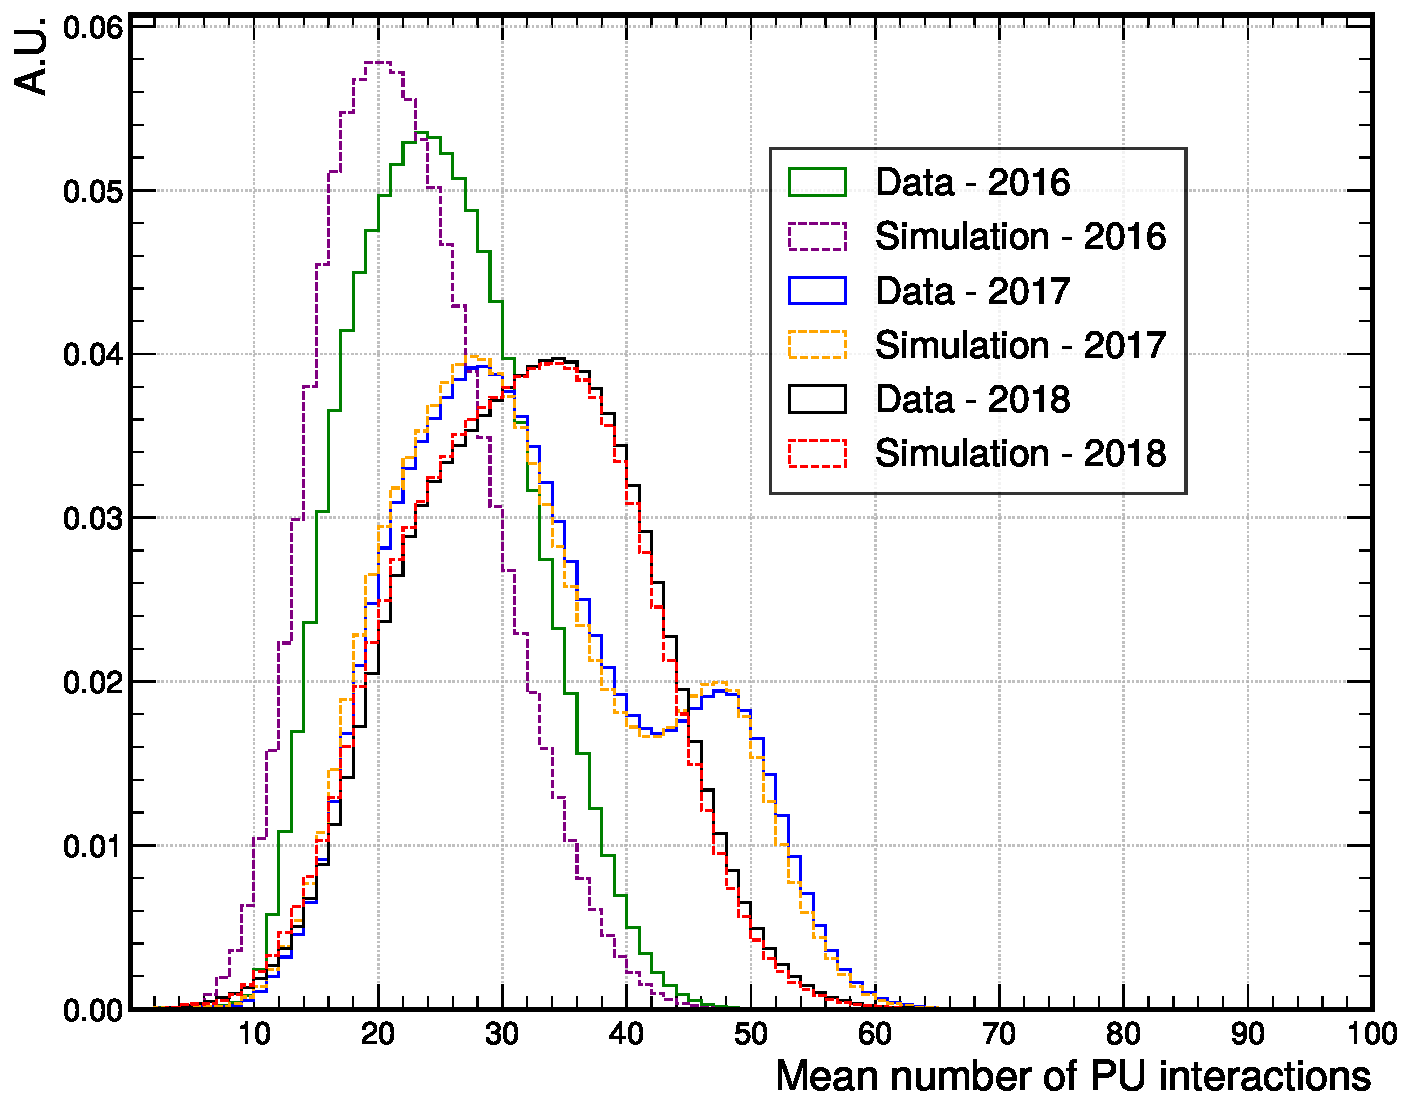
\includegraphics[width=0.8\textwidth]{Figures/Chapter6/PU_Profile.pdf}
\caption{Comparison of the distributions of the mean number of proton-proton interactions per bunch crossing between data and simulation in CMS Run 2.}
\label{Figure:Chapter6_PU_Profiles}
\end{figure}

\subsection{Z $p_\text{T}$/mass Reweighting}

\section{Background Modelling}
\label{Section:Chapter6_Background_Modelling}

\section{Search strategy and statistical procedure}







